\documentclass[handout, 10pt]{beamer}
\usepackage[utf8]{inputenc}
\usetheme{default}
\usecolortheme{dove}
\usepackage{textpos}
\usepackage{grid-system}

% \usepackage[rm]{roboto}
\usepackage[T1]{fontenc}
%\usepackage[sfdefault]{roboto}

% po4a: environment frame
% po4a: environment Row
% po4a: environment Cell

\AtBeginSection[] % Do nothing for \section*
{
	\begin{frame}<beamer>
		\frametitle{Übersicht}
		\tableofcontents[currentsection]
	\end{frame}
}

\title{\centering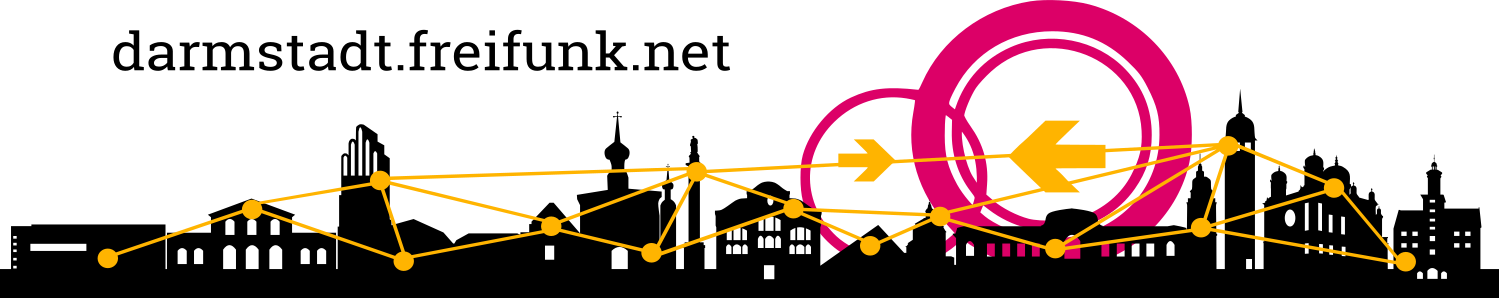
\includegraphics[width=\textwidth]{images/logo-skyline}}
\author{}
%\institute[Inst.]{Freifunk Darmstadt}
\date{\footnotesize 4. Oktober 2015}

\begin{document}


\begin{frame}
\maketitle
\end{frame}

\addtobeamertemplate{frametitle}{}{%
\begin{textblock*}{100mm}(0.92\textwidth,-0.5cm)
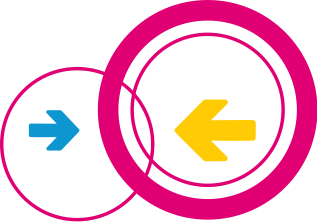
\includegraphics[height=1cm]{images/logo}
\end{textblock*}}

\begin{frame}{Übersicht}
\tableofcontents
\end{frame}

\section{Was ist Freifunk?}
\begin{frame}
	\frametitle{Was ist Freifunk?}

	Deutschlandweite Initiative für freie WLAN-Netze
	
	\pause
	\vfill
	\centering
	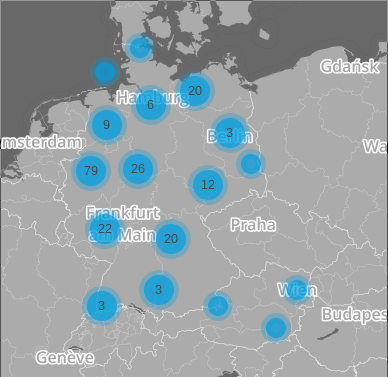
\includegraphics[scale=0.3]{images/2015-10_freifunk-map} \\
	über 200 lokale Gruppen\\bundesweit ca. 20.000 Accesspoints

	
\end{frame}

\begin{frame}
	\frametitle{Wie sieht so ein freies Netz aus?}
	\begin{center}
		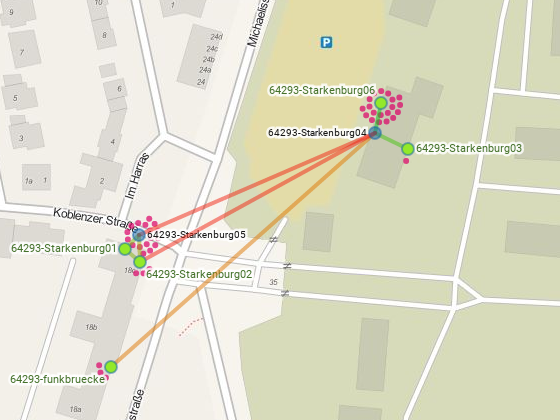
\includegraphics[height=6cm]{images/2015-08-31_starkenburg}
	\end{center}
\end{frame}

\begin{frame}
	\frametitle{Wie sieht so ein freies Netz aus?}
	\begin{center}
		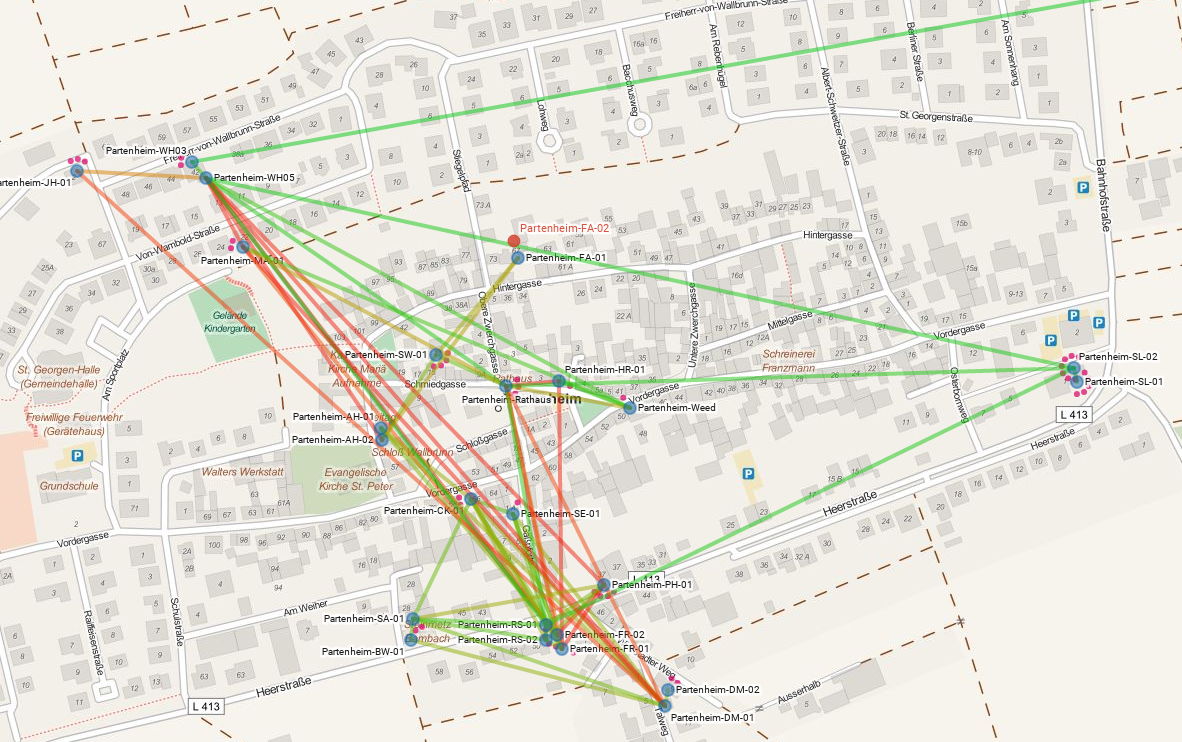
\includegraphics[height=6cm]{images/2015-10_partenheim-map}
	\end{center}
\end{frame}

\begin{frame}{Was kann man damit tun?}
	\vfill
	\begin{center}
		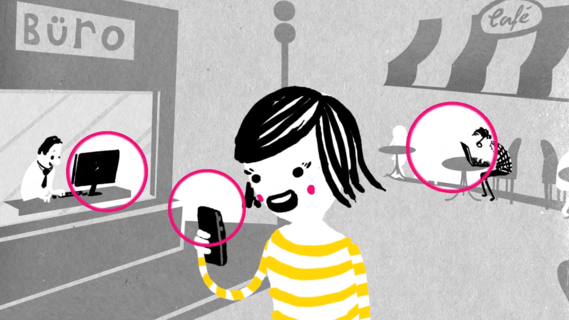
\includegraphics[width=5.5cm]{images/verbindet}
	\end{center}
	
	\begin{itemize}[<+->]
		\item jeder kann Services anbieten und nutzen
		\begin{itemize}
			\item Telefonieren und Chatten
			\item dezentrales Social-Media (z.B Diaspora, Twister)
			\item lizenzfreies Community-Radio
			\item Austausch von Dateien und Medien
			\item \ldots
		\end{itemize}
		\item gemeinsame Nutzung eines Internetanschlusses
		\item Testbed f\"ur wissenschaftliche Experimente
	\end{itemize}
	\vfill
\end{frame}

\begin{frame}
	\frametitle{Vision}
	
	Wie soll unsere Kommunikationsinfrastruktur aussehen?
	
	\begin{itemize}[<+->]
		\item öffentlich
		\item anonym zugänglich
		\item nicht kommerziell
		\item unzensiert
		\item dezentral organisiert
		\item im Besitz einer Gemeinschaft
	\end{itemize}
\end{frame}

\begin{frame}
	\frametitle{Vision: offen und öffentlich}
	
	\begin{itemize}[<+->]
		\item freie, ungehinderte Teilnahme an Betrieb und Ausbau des Netzes $\rarrow$ Mitmachnetz!
		\item freier Zugang zu Netz und Diensten (keine Unterscheidung nach Ort oder Geldbeutel)
	\end{itemize}
	% Bilder: Zugänglichkeit, Menschengruppe mit Notebooks, etc
\end{frame}

\begin{frame}
	\frametitle{Vision: anonyme Zugänglichkeit}
	
	\begin{itemize}[<+->]
		\item Das bedeutet nicht, dass Freifunk Netze den Datenverkehr anonymisieren.
		\item Achtung: Freifunk ist kein Anonymisierungsdienst (wie z.B. Tor), Zuordnung der Daten zu Person deutlich einfacher möglich!
		\item (Verschlüsselung nicht vergessen)
	\end{itemize}
	% Bilder: Tor, Schlüssel
\end{frame}

\begin{frame}
	\frametitle{Vision: Dezentralität}
	
	\begin{itemize}[<+->]
		\item keine zentralen, für die Funktion des Netzes erforderlichen Funktionen
		\item keine Abhängigkeit von einer Gruppe von Personen
		\item allerdings: Zugang zum Internet an mehreren, von ffda betriebenen, Knotenpunkten
		\item Updates der Knoten durch ffda nach Zustimmung durch die Betreiber
	\end{itemize}
	% Bilder dezentrales mesh, zustimmung
\end{frame}

\begin{frame}
	\frametitle{Vision: unkommerzieller Netzbetrieb}
	
	\begin{itemize}[<+->]
		\item kostenloser Zugang zum Netz
		\item kostenloses Meshing mit anderen Knoten und auch Freifunk-Gruppen
		\item Finanzierung der zentralen Gateways ins Internet durch Spenden
				%Bilder Geld, kein Geld, Spende, offene Hand
	\end{itemize}
\end{frame}

\begin{frame}
	\frametitle{Vision: Privatsphäre erhalten}
	
	\begin{itemize}[<+->]
		\item kein sammeln von Verbindungs- oder Verkehrsdaten
		\item keine persönlichen Stammdaten
		\item freiwillige Angabe von Kontaktdaten und Ort eines Knoten
		\item Erhebung statistischer Daten zu Netz- und Knotenauslastung
	\end{itemize}
	% Bilder Privatsphäre, VDS, Datenschutz
\end{frame}

\begin{frame}
	\frametitle{Ziele von Freifunk}
	\begin{itemize}[<+->]
		\item Vermittlung von Verständnis und Wissen zum Betrieb von Datennetzen
		\item Aufmerksamkeit gegenüber gesellschaftlichen Auswirkungen
		\item Beteiligung auch technisch weniger interessiert Menschen an 
		\item Forschung, Entwicklung und Aufbau dezentraler Netze für alle zugänglich machen
		\item Wissen und Software öffentlich zugänglich machen
		\item Beteiligung an politischen Prozessen, um die rechtlichen Voraussetzungen für freie Netze zu schaffen
	\end{itemize}
\end{frame}


\section{Freifunk in Darmstadt}

%Radiostationen, Filmkanäle, Telefoniedienste, Blogs,

%\begin{frame}{Warum Freifunk?}
%\begin{center}\includegraphics[width=0.8\textwidth]{why}
%\vfill
%\pause We need private, free communication!

%Note for translation: private in terms of privacy, not ownership! :P )
%\end{center}
%\end{frame}

\begin{frame}{1.x Jahre FFDA-Netz}
	\vfill
	\begin{itemize}[<+->]
		\item 13. Februar 2014: erstes Treffen
		\item 26. Juni 2014: erster Knoten geht Online
		\item vor einem Jahr: ca. 30 Knoten
	\end{itemize}
	\pause
	\begin{center}
		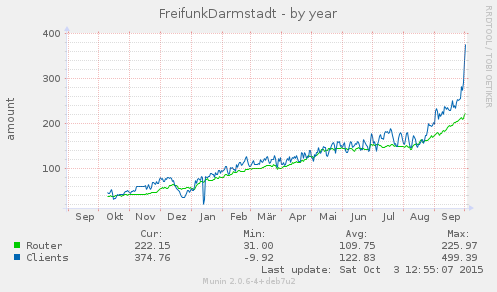
\includegraphics[width=0.8\textwidth]{images/ffda-Okt14-15}
	\end{center}
\end{frame}

\begin{frame}{Stand Oktober 2015}
	\begin{center}
		\vfill
		ca. 220 Knoten, über 400 Clients
		\begin{center}
			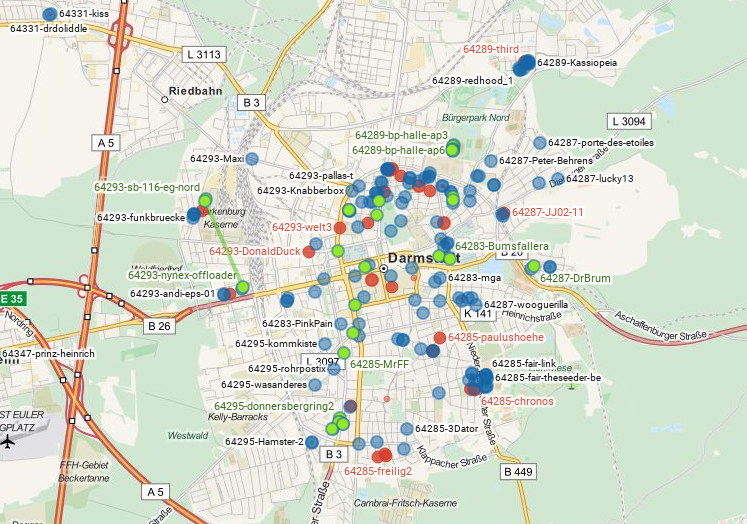
\includegraphics[width=0.7\textwidth]{images/2015-10-03_darmstadt-map}
		\end{center}

		\vfill
		\url{https://map.darmstadt.freifunk.net}
		
		\tiny oder \url{https://map.ffda} im Freifunk-Netz
	\end{center}	
\end{frame}

\begin{frame}{Aktuelle Aufgaben}
	\begin{center}
		\large Flüchtlingsheime mit Internet versorgen \\
		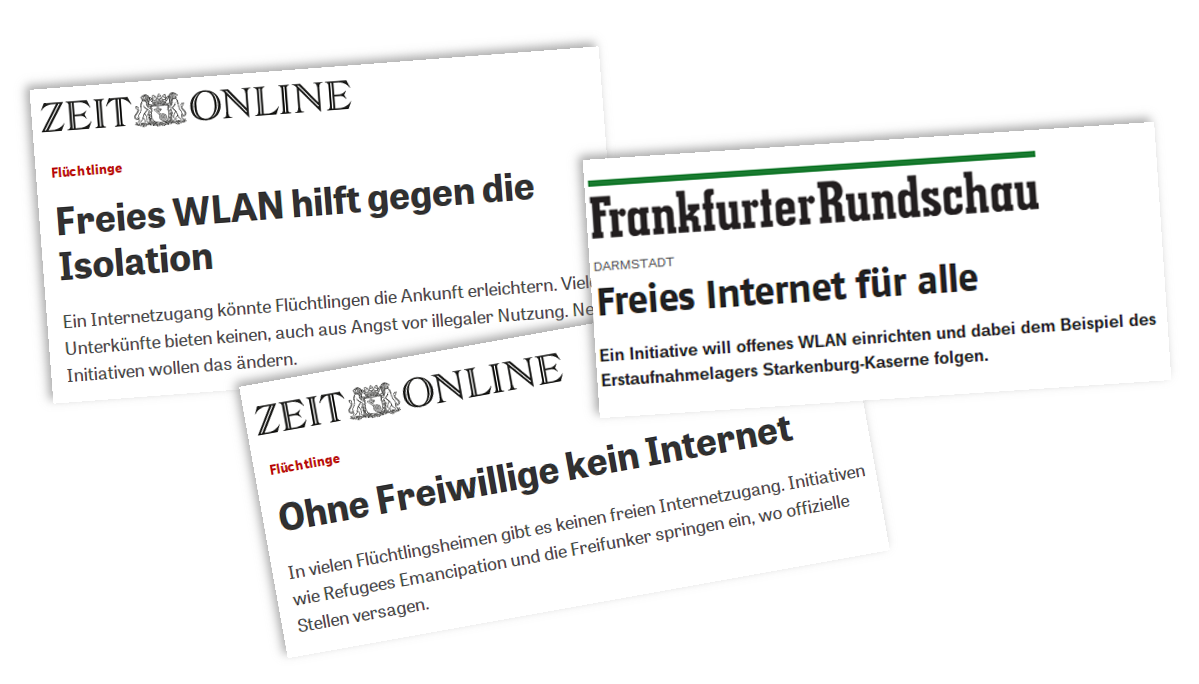
\includegraphics[width=0.7\textwidth]{images/2015-10_presse-fluechtlinge}
	\end{center}
	\begin{itemize}[<+->]
		\item in Darmstadt: Starkenburg Kaserne, Donnersbergring, Sporthalle am Nordbad
		\item auch in Eberstadt, Biebesheim, Stockstadt am Rhein
		\item hoffentlich bald: Seeheim-Jugenheim, Wixhausen, Mühltal
	\end{itemize}	
\end{frame}	

\begin{frame}{Aktuelle Aufgaben}
	\begin{center}
		\large Öffentlichkeitsarbeit
		\vfill
	\end{center}
	\begin{itemize}[<+->]
		\item Kontakt mit:
		\begin{itemize}[<+->]
			\item NGOs, Vereine, Schulen, \ldots
			\item Cafés, Hotels, Geschäfte, \ldots
			\item politische Parteien
			\item Presse
			\item Bewohner
		\end{itemize}	
		\item Vorträge und Workshops organisieren
		\item Sponsoren finden für Technik und öffentliche APs
	\end{itemize}
\end{frame}

\begin{frame}{Aktuelle Aufgaben}
	\begin{center}
		\large Netzwerkwartung
		\vfill
	\end{center}
	\begin{columns}[T]
		\begin{column}{5cm}
			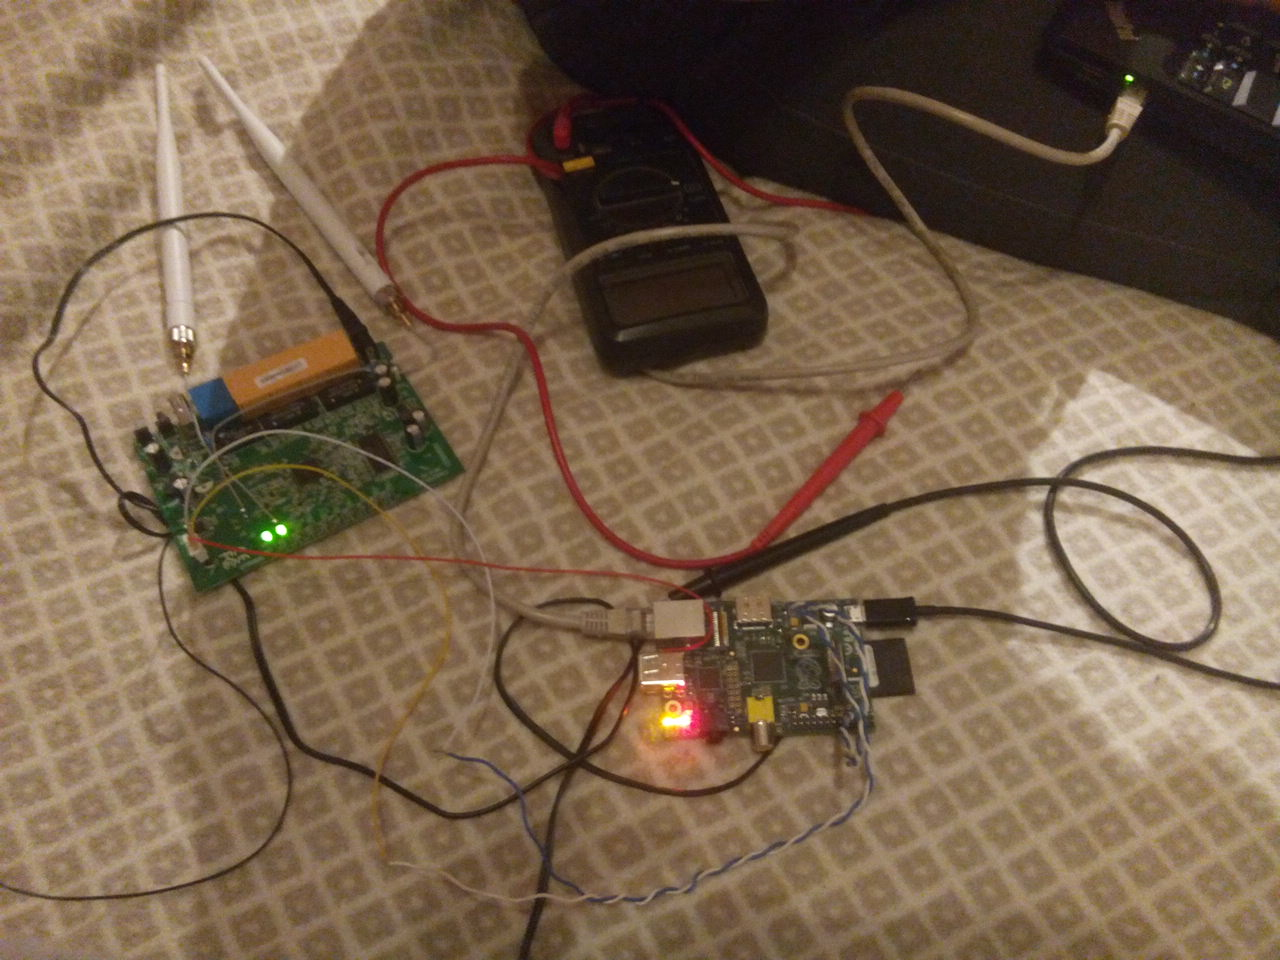
\includegraphics[width=\textwidth]{images/disassemble}
		\end{column}
		\begin{column}{7cm}
			\begin{itemize}[<+->]
				\item neue Firmware für Knoten
				\item Analyse des Netzwerkstatus und Reaktion bei Problemen
				\item Betrieb der Gateways ins Internet
				\item Verbindung zu anderen Communities
				\item Experimente mit unterschiedlichen Protokollen, Software und Hardware
			\end{itemize}
		\end{column}
	\end{columns}
\end{frame}

\section{Wie funktiniert Freifunk?}

\section{Rechtliche Aspekte und Risiken}
\begin{frame}{Rechtliche Aspekte und Risiken}
\begin{Row}
\begin{Cell}{1}
\vspace{0.1cm}

\includegraphics[width=3.7cm]{images/recht}
\end{Cell}
\begin{Cell}{2}
\vspace{1cm}
Überblick:
\begin{itemize}
\pause \item Störerhaftung
\pause \item Risiken fürs eigene Netz
\pause \item Sicherheit im Freifunk-Netz
\pause \item was Freifunk (noch) nicht bietet
\end{itemize}
\end{Cell}
\end{Row}
\end{frame}

\begin{frame}{Störerhaftung}
\begin{itemize}
\pause\item Teilen des eigenen Internetanschlusses ist in Deutschland legal
\begin{itemize}
	\pause\item \textbf{aber:} Mithaftung für illegale Aktivitäten, wenn Täter nicht zu ermitteln ist
\end{itemize}
\pause\item Abmahnkosten sind zu tragen
\vfill
\pause\item aktuelle Lösung: VPN in Länder ohne Störerhaftung
\pause\item Zukunft: selbst Internetanbieter werden
\end{itemize}
\vfill
\centering
\pause \textbf{Fazit:}\\Störerhaftung existiert noch, wir machen es aber sehr schwer,\\den eigentlichen Anschlussinhaber zu finden.

\end{frame}

\begin{frame}{Risiken fürs eigene Netz}
\vfill
\begin{center}
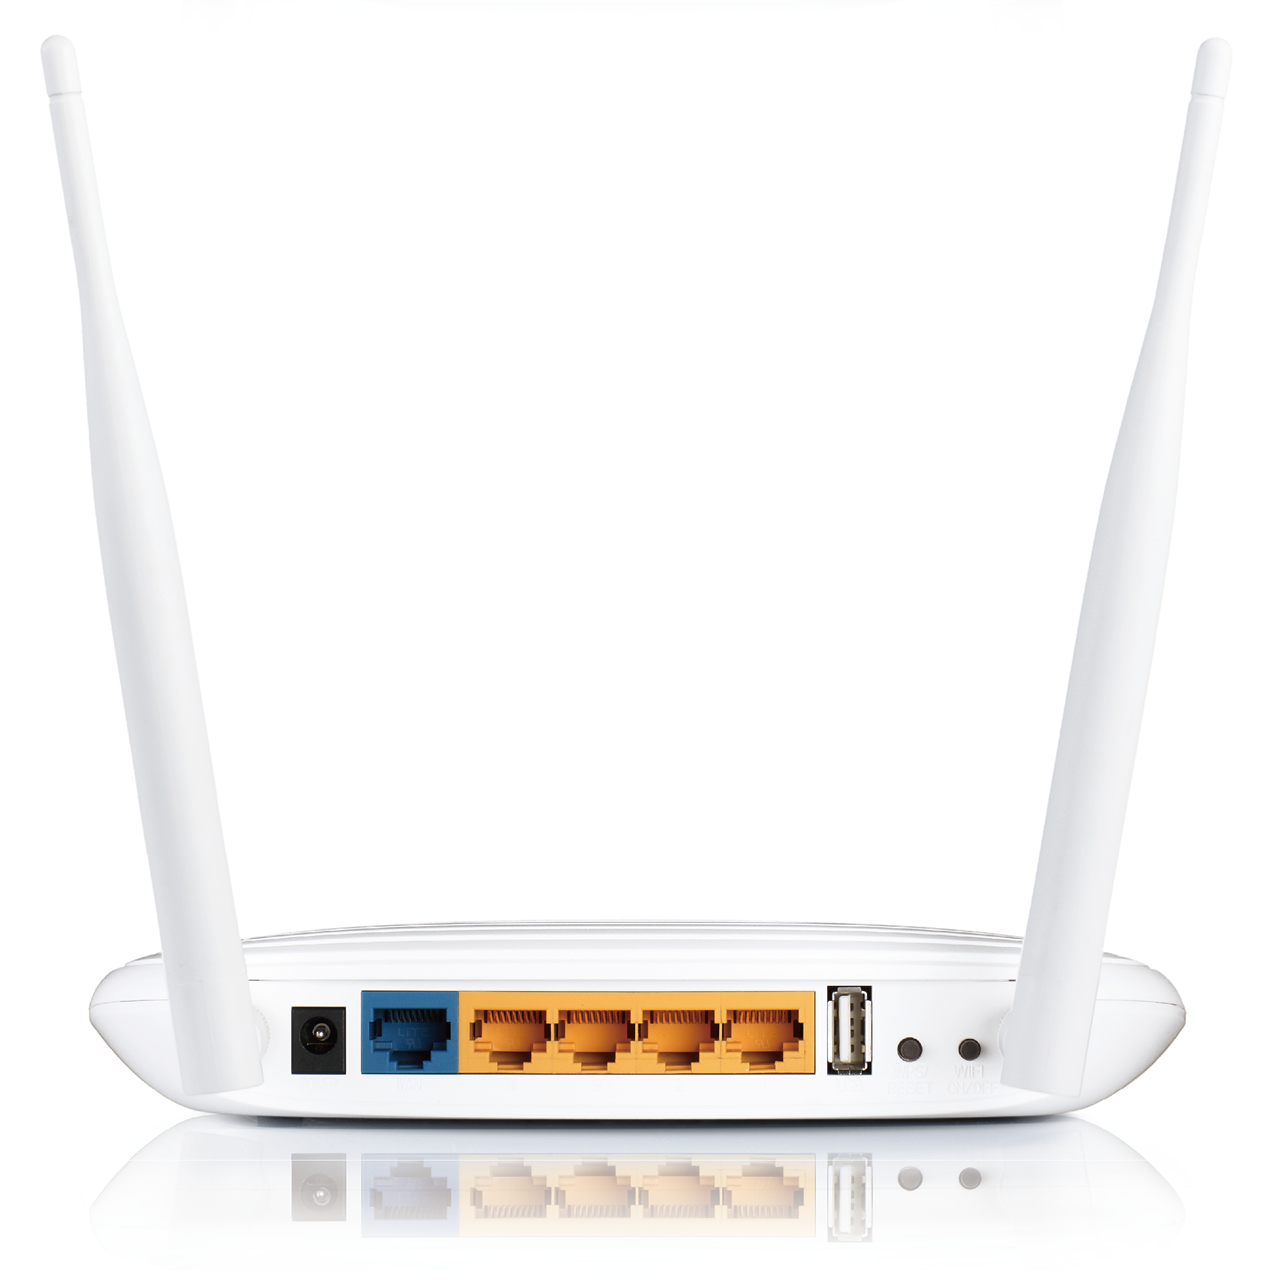
\includegraphics[height=4cm]{images/WR842ND-back}
\end{center}
\begin{itemize}
\pause\item Datenverkehr getrennt
\pause\item eigener Internetzugang nur für VPN zu anderen Knoten im Freifunk-Netz
\pause\item eigenes Netz und Freifunk-Netz sind getrennt, so lange Firmware keine Fehler hat oder gehackt wird
\end{itemize}
\vfill
\end{frame}

\begin{frame}{Sicherheit im Freifunk-Netz}
\begin{itemize}
	\pause\item Freifunk als freies Netz hat wenige Einschränkungen
	\pause\item Menschen können darin auch böse Dinge tun
	\vfill
	\pause\item Daten im Freifunk-Netz: Gesamter Verkehr schwer zu überwachen, aber nicht verschlüsselt
	\pause\item Daten ins Internet: Betreiber der Gateways können überwachen
	\vfill
\pause\item \textbf{Achtung:} WLAN ist nicht verschlüsselt, vertrauliche Daten nur mit Ende-zu-Ende-Verschlüsselung (z.B. https) übertragen
\vfill
\end{itemize}
\centering
\textbf{Fazit:}\\Zentrale Überwachung und Zensur deutlich schwieriger \\ als im Internet
\end{frame}


\begin{frame}{Was Freifunk (noch) nicht bietet}
\vfill
\begin{itemize}
\pause\item Schutz vor Trojanern, Phishing und anderen Gefahren des freien Datenverkehrs
\begin{itemize}
\pause\item[$\rightarrow$] wird es nicht geben, sonst ist es kein freier Datenverkehr mehr
\end{itemize}
\vfill
\pause\item Verschlüsselung gibt es nicht auf allen Teilen der Infrastruktur
\vfill
\pause\item Experimente mit verschlüsseltem Meshing und WLAN AP
\end{itemize}
\vfill
\end{frame}

\begin{frame}{Q~\&~A}
\vfill
\centering
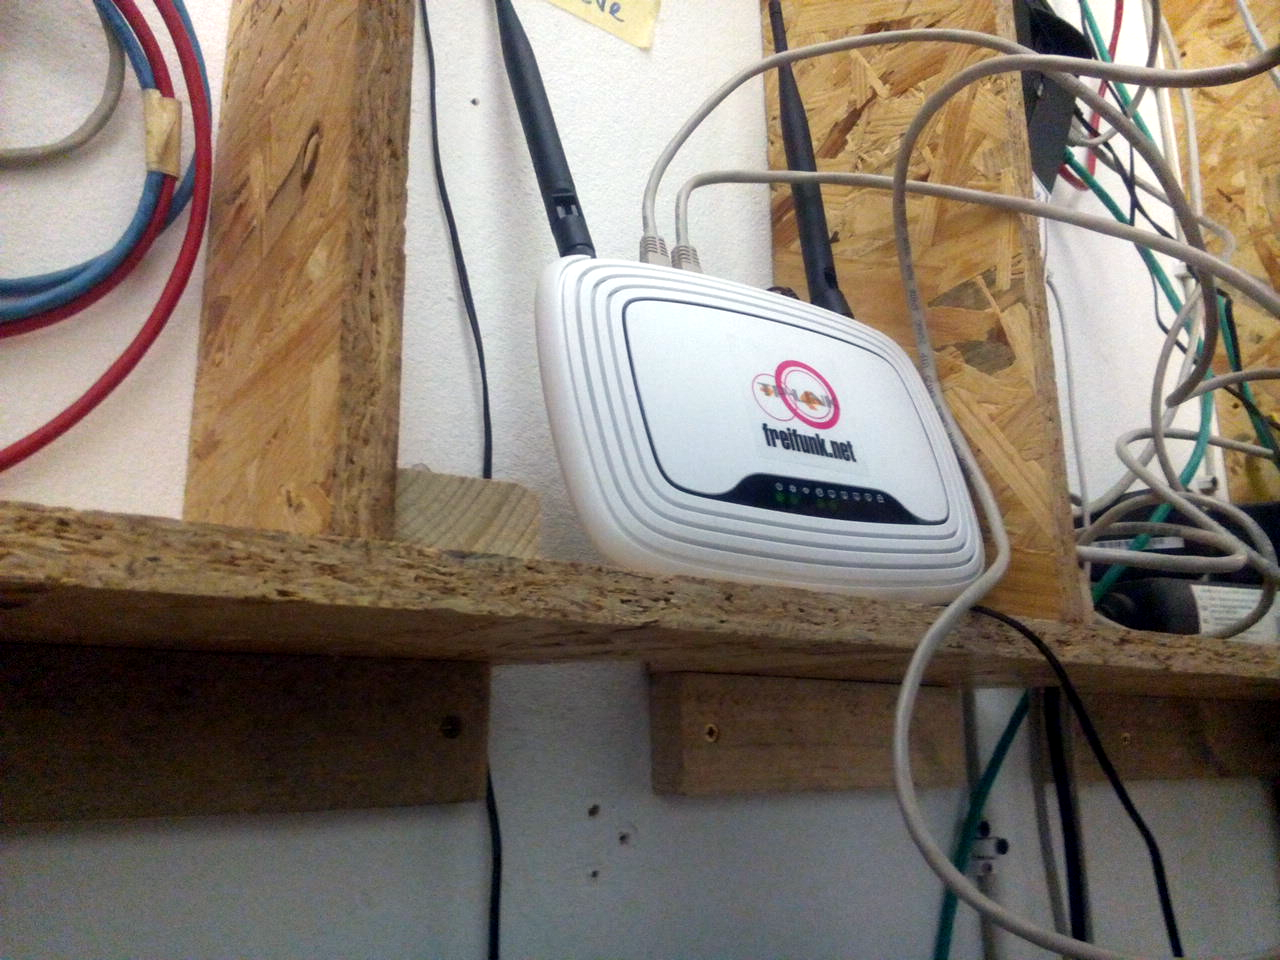
\includegraphics[width=0.7\textwidth]{images/irl_router}
\vfill
\end{frame}


\end{document}
